\documentclass[runningheads]{llncs}

\usepackage{cite}
\usepackage{amsmath,amssymb,amsfonts}
\usepackage{algorithmic}
\usepackage{graphicx}
\usepackage{textcomp}
\usepackage{xcolor}
\usepackage{listings}

\def\BibTeX{{\rm B\kern-.05em{\sc i\kern-.025em b}\kern-.08em
    T\kern-.1667em\lower.7ex\hbox{E}\kern-.125emX}}

\begin{document}

\title{Ensemble Prediction: Computing Accuracy Using Bootstrapping And Bagging Model }
%
%\titlerunning{Abbreviated paper title}
% If the paper title is too long for the running head, you can set
% an abbreviated paper title here
%
\author{Aridaman Singh Nandan \and
Sanjiu Raja Brahma\and
Dr. Nonita Sharma}

\authorrunning{Aridaman et al.}
\institute{Department of Computer Science and Engineering, Dr. B R Ambedkar National Institute of Technology, Jalandhar, Punjab                 
\\
\email{aridamansn.cs.18@nitj.ac.in} \\
\email{sanjiurb.cs.18@nitj.ac.in} \\
\email{nsnonita@gmail.com}} 
%
\maketitle              % typeset the header of the contribution
%
\begin{abstract}
Forecasting models are of many types. Difference lies in the way of generation of forecast, amount of data they use and their complexity. In this paper we have analysed some forecasting methods that could effectively fit on time series to capture the data. Our dataset consist of FCI wheat stock of Punjab region. We applied forecasting techniques to this data to get some predictions and then improved the accuracy of models using ensemble methods: bootstrapping and bagging. To evaluate forecast accuracy and to compare among different models fitted to time series, we have used mean percentage error as a performance measure.

\keywords{Time series  \and Forecasting \and Ensemble Methods \and Bootstrapping \and Bagging.}
\end{abstract}
%
%
%
\section{Introduction}
The aim of time series modelling is to collect the past observations and develop a model which describes the structure. The model should be properly and carefully chosen to fit the underlying time series. Efforts have been done for developing efficient models to improve accuracy of forecasting. Most popular time series modelling technique is Autoregressive Integrated Moving Average (ARIMA); considers time series to be linear. For seasonal time series SARIMA, a variation of ARIMA model is used. Also Artificial Neural Networks (ANN) proved successful for classification and forecasting purposes. ANNs have capability to model non-linear data which is not following any statistical distribution. Two models are generally used for time series:
\begin{itemize}
\item Multiplicative model: \begin{equation}
	Q(t) = Tr(t) {\times} Ss(t) {\times} Cy(t) {\times} Irr(t) 
\end{equation}
\item Additive model: \begin{equation}
   Q(t) = Tr(t) + Ss(t) + Cy(t) + Irr(t) 
\end{equation}
\end{itemize}
Here Q(t) is observation, Tr(t) is trend, Ss(t) is seasonality, Cy(t) and Irr(t) is cyclic and irregular variation.
Multiplicative model is based on assumption that time series can affect one another i.e. not necessarily independent. Additive model assumes components are independent of each other.
%
%
%
\section{Time-Series Forecasting}
Time series can be defined as an ordered sequence of values of a variable at equally spaced time intervals [1]. Time series models obtains details of forces and structure exhibited by observed data. Classical approaches decompose the time series into trend, seasonal and residual components. Before applying models data is examined and if necessary, some transformations are applied to be able to interpret the series better. This can stabilize the variance. For example, if there is trend in the series then logarithmic transformation is suggested. If there are outliers they need to be adjusted.
\linebreak Time series is classified into two types:
\begin{itemize}
\item Univariate- means you have the time-stamp, and you have one variable connected to the time-stamp. For univariate datasets we have common statistics like mean and variance.
\item Multivariate- is like a metric with several variables attached to time-stamp.
\end{itemize}
The fitting of a model is an ambitious undertaking. Many kind of models are there. Data stationarity is a common assumption in many time series techniques. Stationarity is a key trait when it comes to working with time data. Basically the question behind it is- has the data the same statistical properties throughout the time series? Stats properties which determine stationarity contain variance, mean and autocorrelation. Discussion on these models is done in [5,6,9,8].
%
%
%
\section{Preparation Of Data}
To make some predictions about the future the data has to be time series. For this project we used the FCI wheat stock data of Punjab region which had daily wheat stock record for the year 2017 [2] The dataset contains the daily observations of commodity stocks.
 \paragraph{Converting to univariate} The acquired dataset was multivariate as it contained data of multiple sub-regions of Punjab whereas our analysis required data from only one sub-region. Thus, we first removed the data related to other sub-regions and made it a univariate dataset. 
\paragraph{Removing attributes} We removed the attributes which were of no use in the forecasting process like the sub-region identifier ID and many more. Only contributing attributes in the forecasting were kept.
\paragraph{Converting to ts} We used the ts() function of R[3] to create time series object of vector dataset. The data was sampled at equispaced points in time.
\paragraph{Decomposing} The data had trend in it, and we found change in mean as a result of trend. Predictions tend to be underestimated as a result of this. One solution to the problem is to de-trend the data[4]. Thus, data was decomposed into single components[5], removed the trend component, and checked for trend stationarity. This was not enough and differencing was used, which gives difference stationarity.
\paragraph{Data cleaning} Outliers induce biasing in forecasting models. They are unusual or may be errors.  tsclean() function identifies and replaces outliers[8]. Other way could be logarithmic transformation[9].
\paragraph{Testing Stationarity} Unit root tests can be used to check for trend stationarity or difference stationarity. The most prominent of these test is the augmented Dickey-Fuller test[6]. The adf.test() function in R[7] performs this test for null hypothesis of a unit root on a univariate ts. It removes autocorrelation before it tests for stationarity.

Now that the data is converted into a form that is suitable for accurate predictions, we move to forecasting methods. In next section we discuss about different forecasting techniques.
\begin{figure}
\centering
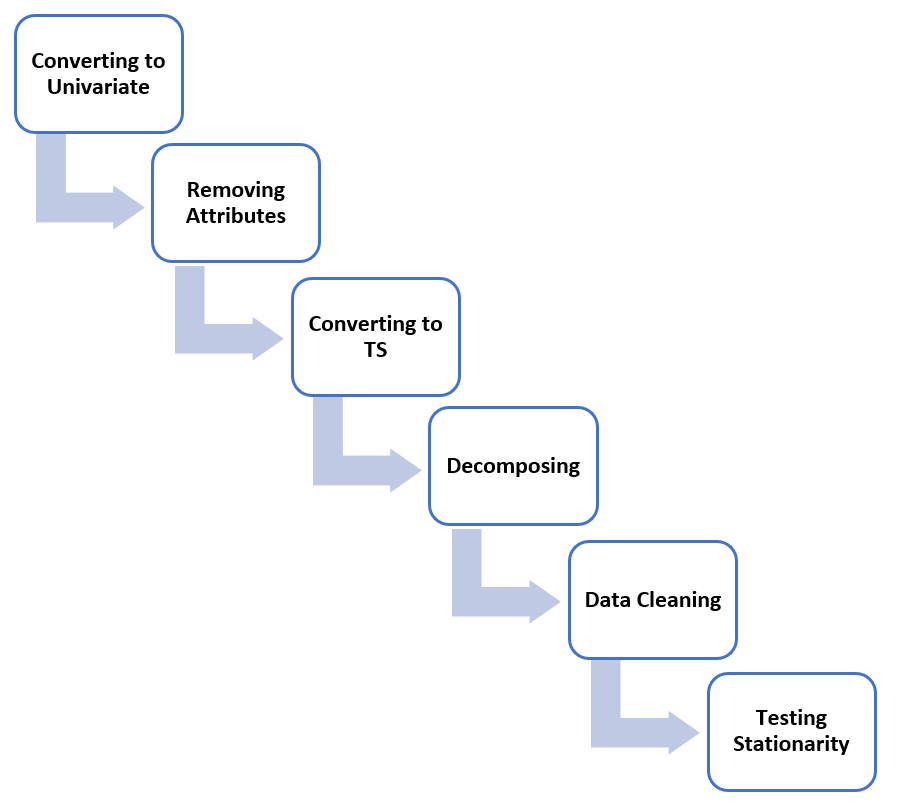
\includegraphics[scale=1,width=10cm,height=6cm]{chart.png}
\caption[20]{Steps in preparing the data}
\end{figure}
%
%
%
\section{Time Series Models And Forecasting}
Interestingly, simple and primitive forecasting methods can outperform advanced models in certain circumstances. If dataset is random, then its hard with models like ARIMA and exponential smoothing. The beauty of advanced models is that they can exploit patterns really well. The idea of forecasting model is to exploit one obvious fact. The fact can be the last observation, it can be the mean, or it can be the general trend.
\linebreak
Forecasting methods involves several approaches to predicting uncertain events. Such system requires identifying forecasting problems, implementing a range of forecasting methods, making an appropriate selection for each problem and refining forecasting methods by evaluation over time[10].

\subsection{Basic Forecasting Models: Mean, Naive And Drift}
These models carry the observations forward. Last observations are projected into the future. The naive method can be tweaked so that it can work with seasonal dataset. Last observations of same seasonal stage are projected. Another simple method is average or mean which simply calculates the mean of data. Forecast of future values is equal to mean of historical data. Drift method calculate the increase between the first and last observation and carry the increase to the future.
\begin{figure}
\centering
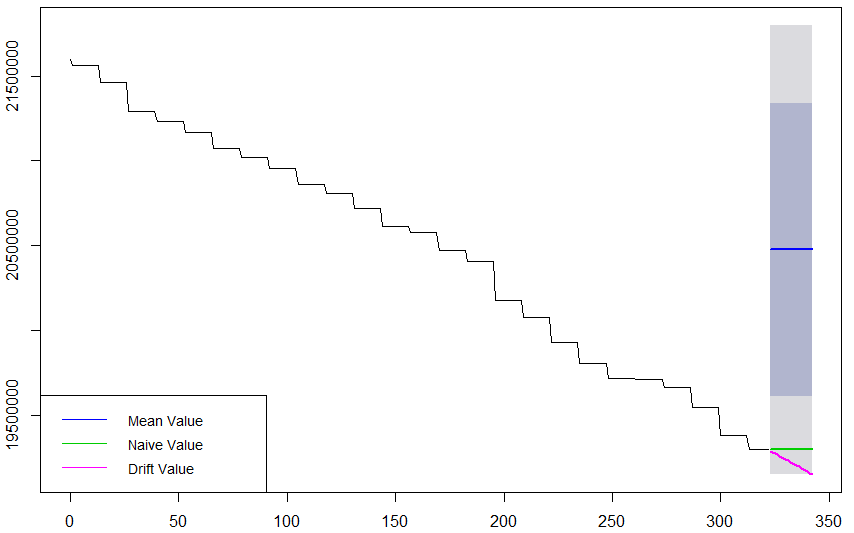
\includegraphics[scale=1,width=10cm,height=5cm]{BasicModelsNew.png}
\caption{Basic Models: Mean, Naive and Drift model forecast for next 20 days}
\end{figure}
Figure 2 shows the predictions based on these models.


\subsection{ARIMA}
ARIMA describe autocorrelation present in data. Seasonality and trend affect the time series at different intervals. ARIMA requires time series to be stationary whose properties do not depend on time at which series was observed.
\linebreak
Differencing makes non stationary time series stationary. It computes differences in observations. Differencing stabilize the mean and therefore, trend and seasonality are either removed or reduced. Mathematically it is described as-
\begin{equation*}
  y(t) = y(t) - y(t-1) 
\end{equation*}
The new series will have T - 1 values. Second order differencing can also be used if first order differencing is not satisfactory.
ARIMA has three parameters:
\begin{itemize}
\item p : number of lags used in the model. It refers to the previous values used in the regression equation.
\item d : used to stabilize the series when not stationary.
\item q : moving average component represents the error of the model with combination of previous error.
\end{itemize}

The whole model is summation of lags. R has auto.arima() function that does the differencing automatically and calculate the parameters whereas the arima() function requires the parameters to be passed. Figure 3 and 4 shows the model with different parameters.

\begin{figure}
\centering
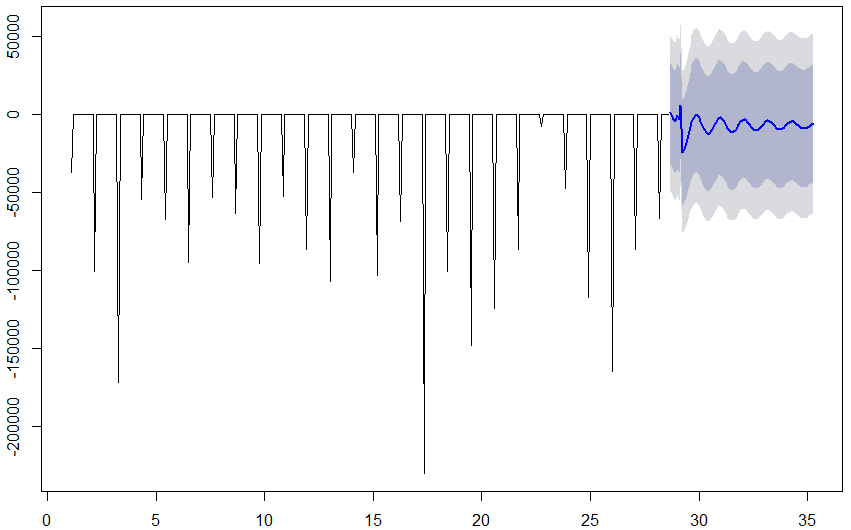
\includegraphics[scale=1,width=10cm,height=5cm]{ArimaNew.png} 
\caption{Forecast from auto.arima() model(3,0,3) fitted to stabilized commodity stock}
\end{figure}

\begin{figure}
\centering
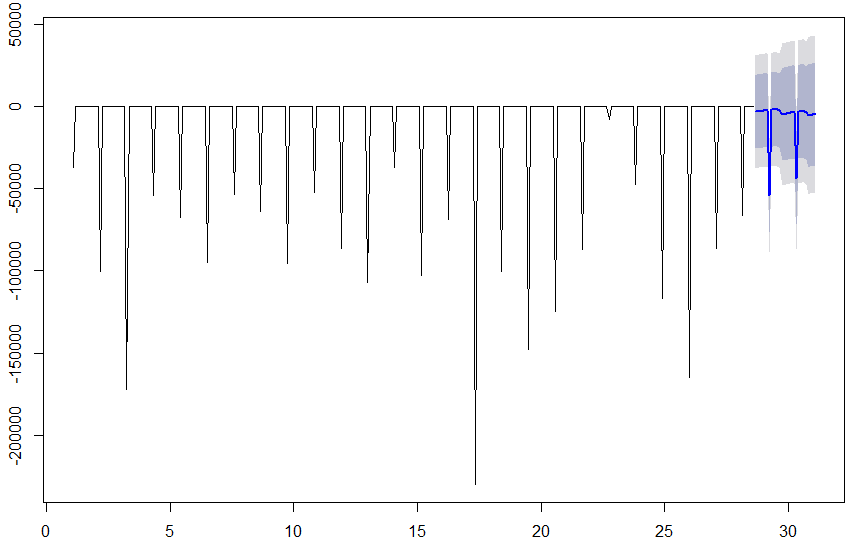
\includegraphics[scale=1,width=10cm,height=5cm]{Arima!AutoNew.png} 
\caption{Arima provided with parameters p=13, d=0, q=4}
\end{figure}

\subsection{Exponential Smoothing}
Exponential smoothing weight the previous observations by decreasing weights as the observations get older. Old data is considered as less relevant and progressively more weight is assigned to newer data. It ignores the deviations irrelevant to the purpose and hence can be used as a forecasting method to forecast data with no clear trend or seasonality. Moving average assigns equal weight of 1/N of all observations. In exponential smoothing to assign weights  to the observations there are some smoothing parameters to be estimated.

Simple exponential smoothing decreases weight using weighted moving average. The basic formula is-
\begin{equation}
  S_{t} = {\alpha}z_{t-1} + (1-{\alpha})S_{t-1}
\end{equation}
where a is a value from 0 to 1 called smoothing constant and t is time period. Smoothing happens to be slow if a is close to zero. For data showing trend double exponential smoothing is more reliable:
\begin{equation}
  l_{t} = {\beta}(S_{t} - S_{t-1}) + (1 - {\beta})l_{t-1}
\end{equation}
where beta is a constant which is chosen in reference to alpha.
Model consist of three characters for identifying the method used.
Error type is denoted by first letter, second denotes trend type and third denotes the season type. The type could be "N"=none, "M"=Multiplicative, "A"=Additive and "Z"=automatically.
Figure 5 shows the prediction by additive error exponential smoothing model using ets() function in R.
\begin{figure}
\centering
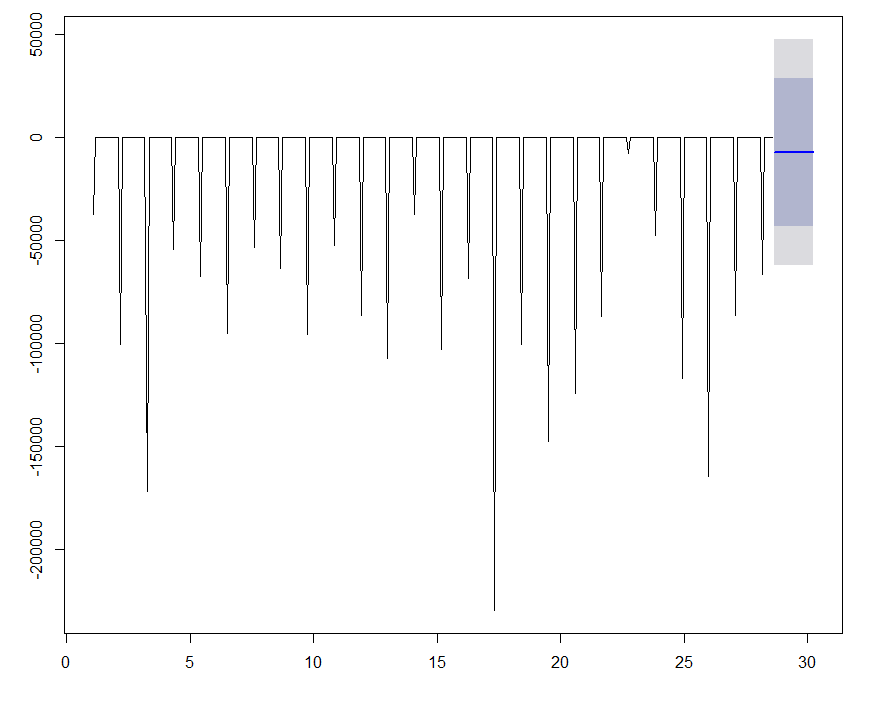
\includegraphics[scale=1,width=10cm,height=5cm]{ets.png} 
\caption{Forecast from ETS(A,N,N)}
\end{figure}

\subsection{Neural Network Model}
It is a statistical model popularly used in machine learning. ANN model works as a brain in a mathematical way. It is a network of neurons organized in layers. Linear combination of the inputs provides the forecast. The output of the hidden layer is modified using a non linear function called sigmoid. This is the associated activation function used to transform the input to an output which in turn acts as input to the subsequent layers.

For NN implementation to be successful proper training on training set is required. This process of training makes the NN system learn to adjust the weights connected with a suitable learning algorithm.

\begin{equation}
s(z) = \frac{1}{1 + e^{-z}}
\end{equation}

\begin{figure}
\centering
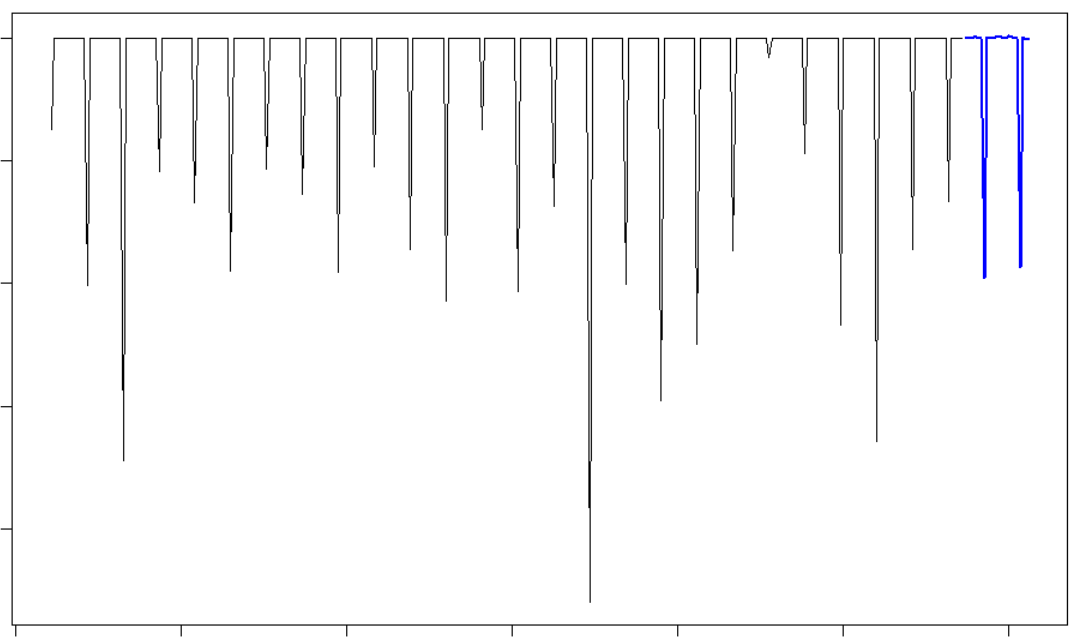
\includegraphics[scale=1,width=10cm,height=5cm]{NNARNew.png} 
\caption{Forecasts from neural network model using nnetar() function in R}
\end{figure}

We use the notation NNAR(p,q) to indicate p lagged inputs and k hidden layer nodes[11][Fig.6]. For example NNAR(7,3) means model is a neural network with last 7 observations.

\subsection{SARIMA}
Seasonal data can also be modelled using ARIMA. It explicitly supports univariate time-series with seasonal component. This is achieved by introducing additional terms in ARIMA. The seasonal part of the model consists of terms that are very similar to the non-seasonal components of the model. The four seasonal elements are: 
\begin{itemize}
\item P: seasonal autoregressive order
\item D: seasonal difference order
\item Q: seasonal moving average order
\item m: number of time steps for a single seasonal period
\end{itemize}

\begin{figure}
\centering
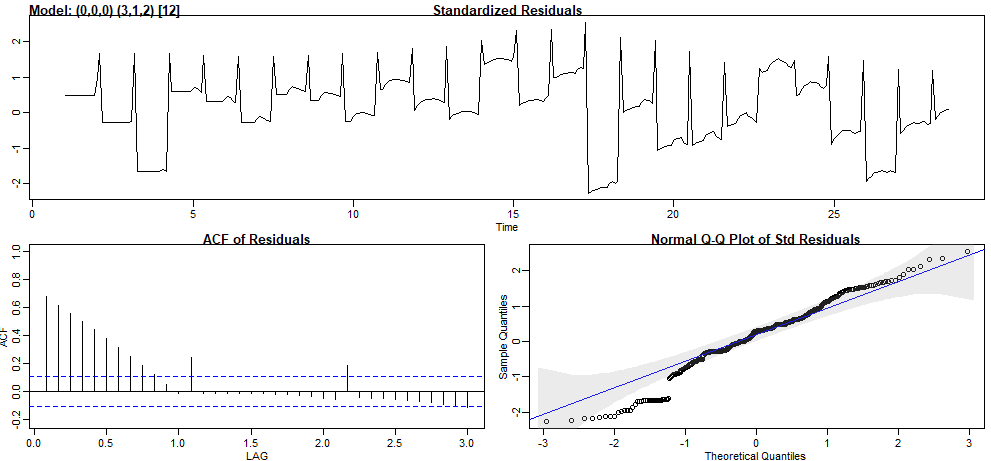
\includegraphics[scale=1,width=10cm]{Sarima.png} 
\caption{SARIMA model diagnostics}
\end{figure}

SARIMA chooses the lag equal to the number of seasons to remove the additive seasonal effects. Using the sarima() function we inspect the model fit diagnostics[13].

Looking at the model diagnostics, we can see that the model does fit fine, although there might still be some outliers in the data with unexplained variance as shown in the Normal QQ plot[Fig.7].
Using the sarima.for() function, we can provide a forecast of the next few time intervals based on our model[Fig.6]. There is a prediction bounds[Fig.8], along with the predicted data. The uncertainty
increases in amplitude as time progresses.





\begin{figure}
\centering
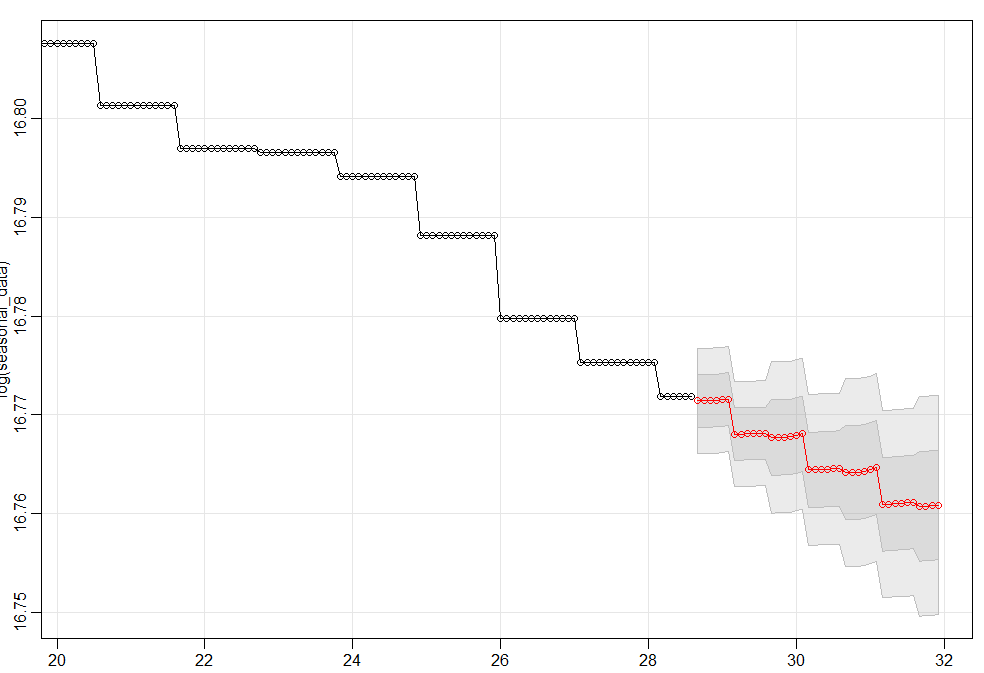
\includegraphics[scale=1,width=10cm,height=5cm]{SarimaPrediction.png} 
\caption{SARIMA forecast prediction for 40 future points}
\end{figure}

\section{Comparing Models Accuracy}
Working on a problem we don't settle on one model, rather on two or more well-performing models. We compare the models by tuning the parameters of each and discover the worst and the best performer. It gives an idea of spread of model or perhaps one can be improved.
The models constructed and tuned here are Arima, exponential smoothing, Neural Network and Sarima. The models are tuned automatically(except Arima) and evaluated using MPE. Once the models are tuned with optimal configurations found for each the accuracy results of best models are collected. Data was partitioned into training dataset used to prepare the model and an unseen test set used to evaluate the model.
The assessment of all methods shown in table 1.
\begin{table}
\centering
\caption{Model accuracy in terms of Mean Percentage Error.}\label{tab1}
\begin{tabular}{|l|l|}
\hline
Forecasting Model &  MPE\\
\hline
Mean &  -5\\
Naive &  -1.01\\
Drift & 1.5\\
Auto Arima & 0.96 \\
Arima(13,0,4) & 0.7\\
ETS & 1.96 \\
NNAR & 0.64 \\
\hline
\end{tabular}
\end{table}

\section{Ensemble Method: Bootstrapping and Bagging}
Time series can be simulated to predict future values by using a model. A similar time series to the observed series can be generated using bootstrapping. We present a method for bootstrap aggregation (bagging) of exponential smoothing methods. Time series is first Box-Cox transformed[15], and decomposed into trend, seasonal and residual components. A bootstrapped remainder series is obtained by shuffling versions of residual components. Contiguous sections of time series are selected at random and joined together. Trend and seasonality components are added and Box-Cox transformation is reversed to original time series.

Bootstrapping is useful in two ways:
\begin{itemize}
\item better measure of forecasting uncertainty.
\item provides a way for improving forecast accuracy by using "bagging"
\end{itemize}

Our focus is on improving the accuracy of forecasting methods. Producing forecasts from each of the additional time series, and average the forecasting result, we get better forecasts than by applying on the original time series directly. This is called bagging. We will use ets() to forecast each of these series. Fig 9 shows ten forecasts obtained in this way.

\begin{figure}
\centering
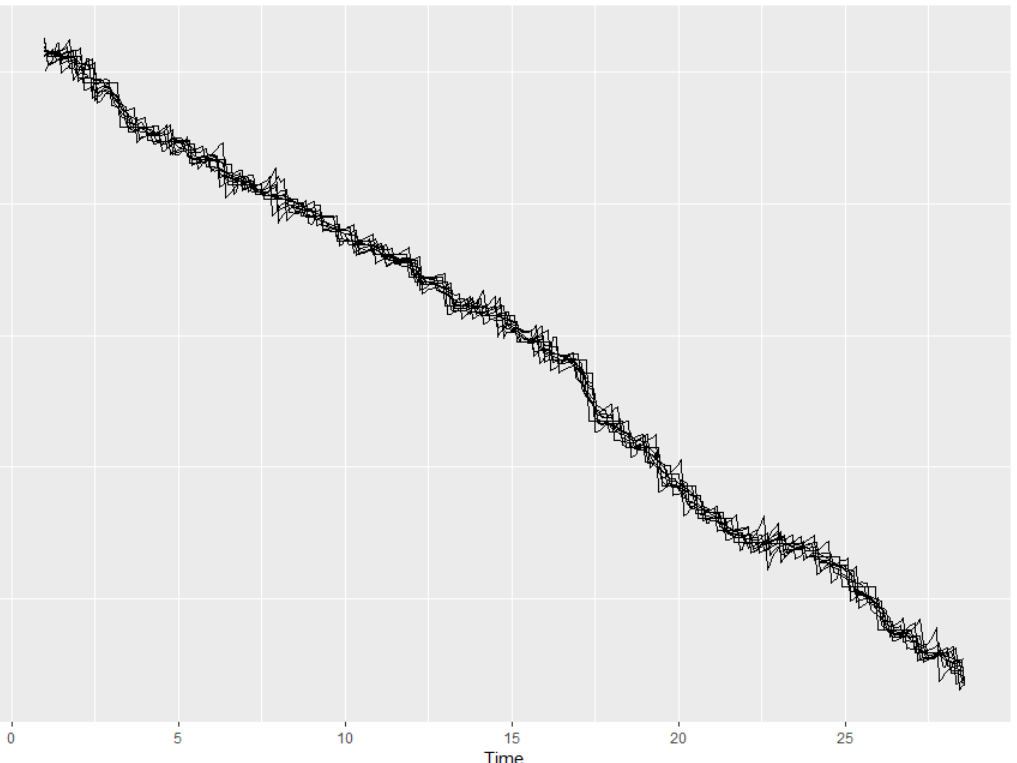
\includegraphics[scale=1,width=10cm,height=5cm]{BootstrappedSeries.png} 
\caption{Bootstrapped version of commodity stock}
\end{figure}

We use the bootstrap() function in forecast package of R to create bootstrapped series. Code snippet shown below creates 10 different bootstrapped series on original data by performing bootstrapping and converting the series into time series objects. Fig. 9 shows 10 different bootstrap series fitted on the original time series. Plot is obtained using autoplot() function in R.
\begin{lstlisting}[language=R]
bs = bld.mbb.bootstrap(data, 10) %>%
  as.data.frame() %>% ts(frequency=12)  
f = purrr::map(as.list(bs),
 function(x){forecast(ets(x))[["mean"]]})
  %>% as.data.frame() %>%
  ts(frequency=12)
\end{lstlisting}

The average of these forecast models gives the bagged forecast of original data. The entire process is handled by baggedETS() function. By default, 100 bootstrapped series are used.

\begin{lstlisting}[language=R]
ets_output = data %>% ets() %>% 
		forecast(h=36)
bagged_output = data %>% baggedETS()
		 %>% forecast(h=36)
\end{lstlisting}
Resulting forecasts are shown in Fig. 10. The difference seems to be very little. But bagging gives better forecast by applying on huge datasets. The method gave MPE of 0.01 on commodity stock dataset and outperformed all other models.



\begin{figure}
\centering
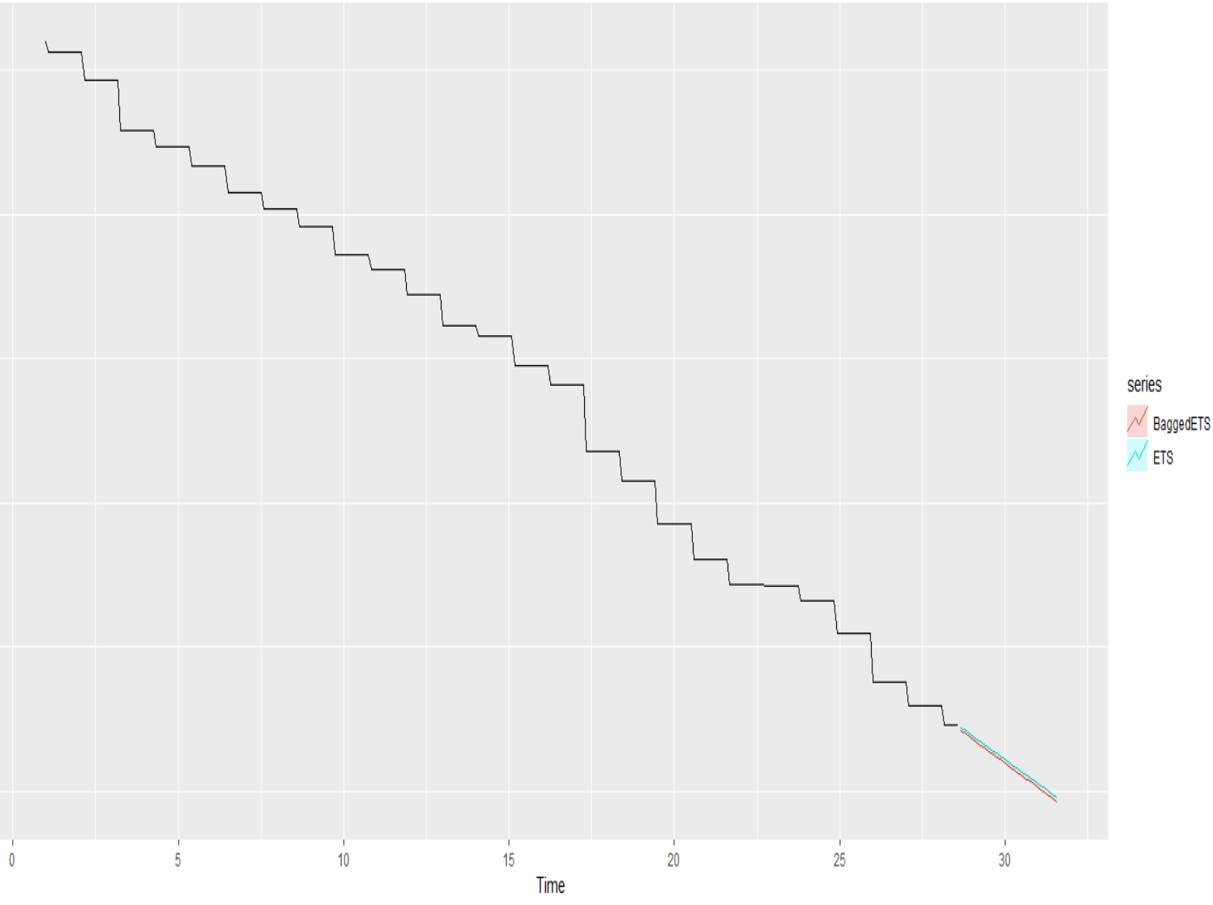
\includegraphics[scale=1,width=10cm,height=5cm]{BaggedETS.png} 
\caption{Bagged ETS forecasts and ETS applied directly to the data.}
\end{figure}

\section{Conclusion}
In this analysis we compared the results from multiple models, with their parameters optimized. Capability of model is evaluated on unseen data. Basic forecasting models are outperformed by advanced methods. Neural network model performed good and exponential smoothing did worst. Improving the accuracy by using ensemble methods on exponential smoothing the error was reduced largely. This is because bagging considers the average of forecast uncertainty to improve forecasting accuracy. It simulates original series by creating dummy series and fit the newly created series on original one hence averaging the result for prediction. It reduce the variance in prediction and improve the stability and accuracy. Of course, it is slower as more computations are required.


\begin{thebibliography}{8}
\bibitem{b1} NIST/SEMATECH e-Handbook of Statistical Methods, http://www.itl.nist.gov/div898/handbook/
\bibitem{b2} Open Government Data(OGD) Platform India,
https://data.gov.in/keywords/fci-stock
\bibitem{b3} ts: Time-Series Objects,

https://www.rdocumentation.org/packages/stats/versions/3.5.3/topics/ts

\bibitem{b4} J. Brownlee, How To Decompose Time Series Data Into Trend And Seasonality,
https://machinelearningmastery.com/decompose-time-series-data-trend-seasonality/
\bibitem{b5} Seasonal Decomposition Of Time Series By Loess-
Decompose a time series into seasonal, trend and irregular components using loess,
https://www.rdocumentation.org/packages/stats/versions/3.6.0/topics/stl
\bibitem{b6} Rob J Hyndman, Unit Root Tests,

https://www.rdocumentation.org/packages/aTSA/versions/3.1.2/topics/adf.test
\bibitem{b7}Augmented Dickey-Fuller Test,

https://www.rdocumentation.org/packages/aTSA/versions/3.1.2/topics/adf.test
\bibitem{b8} Dealing with missing values and outliers,
https://otexts.com/fpp2/missing-outliers.html
\bibitem{b9} Transforming Data,
http://rcompanion.org/handbook/I-12.html

\bibitem{b10}Rob J Hyndman and George Athansopoulos, Forecasting, planning and goals
https://otexts.com/fpp2/planning.html 
\bibitem{b11} Rob J Hyndman and George Athansopoulos, Advanced Forecasting Methods,
https://otexts.com/fpp2/nnetar.html

\bibitem{b12} Debasish Sena1
 and Naresh K. Nagwani, A NEURAL NETWORK AUTOREGRESSION MODEL TO FORECAST
PER CAPITA DISPOSABLE INCOME 
\bibitem{b13} Kenneth Foo, Seasonal lags: SARIMA modelling and forecasting, Jan 3, 2018, 
https://medium.com/@kfoofw/seasonal-lags-sarima-model-fa671a858729
\bibitem{b14}  Kandananond, K. (2012). A Comparison of Various Forecasting Methods for Autocorrelated Time Series. International Journal of Engineering Business Management. https://doi.org/10.5772/51088
\bibitem{b15} Box, G. E. P. and Cox, D. R. (1964). An analysis of transformations, Journal of the Royal Statistical Society, Series B, 26, 211-252.
\end{thebibliography}
\end{document}
